\section{Results and Discussion}
\par
This section contains the result obtained during the design phase of the project.
\subsection{Discharge Flow Control Unit Assembly}
\par
The assembly regulates the discharge flow in precise steps as per the users specifications through the use of a servo motor. Furthermore, to ensure that no sliding of the motor and the motor mounts along the valve, the assembly utilizes the use of serrated straps to enhance grip. The slots in the servo motor holder mount allows for the servo motor to be aligned with the ball valves shaft during setup before the start of the experiment.
\begin{figure}[ht]
    \centering
    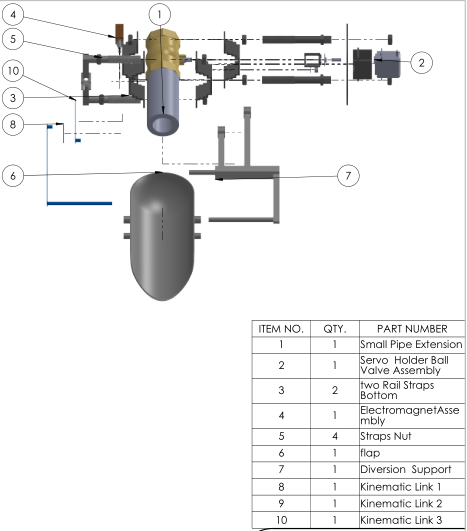
\includegraphics[width=\textwidth,height=0.9\textheight,keepaspectratio]{Figures/assembly.png}
    \caption{Discharge Flow Control Unit and Discharge Collection Unit Assembly}
    \label{fig:assembly}
\end{figure}
\subsection{Discharge Flow Collection assembly}
\par
The sub assembly efficiently and correctly diverts the discharge either to the main collection tank or into the main reservoir through the use of flaps.  This is achieved through the use of an electromagnet. The electromagnet is also correctly positioned to ensure minimal splashes which would otherwise interfere with the electrical components. Furthermore, the fast response of the unit is achieved by the use of an electromagnet whose linear motion is amplified by the use of a lever system hence providing the flap with a wider angle.
\par
Additionally, to ensure that only the required amount of water is collected and there are minimal splashes, the sub assembly uses a curved flap. The weight of the collected discharge is also measured by use of correctly positioned load cells which are evenly distributed at the four edges of the collection tank. The weight values from the four load cells are taken after which the average is computed which is taken as the final weight of the discharge. The use of a horizontal cylindrical tank enhances motivated discharge into the main reservoir, in that the discharge fluid is released within a stipulated time through the use of the solenoid valve. 
\begin{figure}[ht]
    \centering
    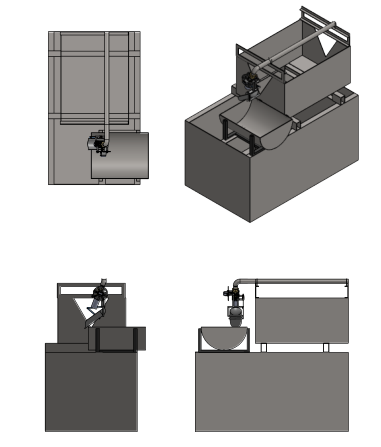
\includegraphics[width=\textwidth,height=0.9\textheight,keepaspectratio]{Figures/final assembly.png}
    \caption{Final Assembly}
    \label{fig:final assembly}
\end{figure}

\clearpage
\subsection{Budget}

\begin{longtable}[!ht]{lllll}
\hline
Item No. & Item & Quantity & Unit cost & Cost \\ \hline
\endfirsthead
%
\multicolumn{5}{c}%
{{\bfseries Table \thetable\ continued from previous page}} \\
\endhead
%
1 & Servo Motor MG996 & 1 & 800 & 800 \\
2 & JF-0530B DC12V electromagnet Push-Pull solenoid & 1 & 550 & 550 \\
3 & 1M/3M DS18b20 temperature probe & 1 & 400 & 400 \\
4 & LCD Touch (ILI9341 driver) & 1 & 1300 & 1300 \\
5 & STM32F407VET6 & 1 & 4300 & 4300 \\
6 & 50Kg Load cells & 4 & 150 & 600 \\
7 & HX711 Weight amplifier & 1 & 50 & 50 \\
8 & 3D printing &  &  & 10000 \\
9 & Miscellaneous & &  & 2000 \\
Total &  &  &   & 20000\\
\hline
\caption{Budget}
\end{longtable}


